% TODO: Table numbering.
\subsection{Motion Segmentation figure: ATE results}
In this section, figure: results for the Motion Segmentation system
to complement those outlined in Section~\ref{sec:moseg_quantitative} are given.
The results in this section assess Absolute Trajectory Error on the TUM Dynamic
Objects \textit{Validation} set. Quantitative results are given in Table
~\ref{table:moseg_ate_validation} and visualised in Figure~\ref{figure:moseg_ate_validation}.

\begin{table}[!htbp]
\begin{center}
  \begin{tabular}{l c c}
    \emph{TUM Standard Sequence Name} & \emph{MoSeg} ATE (m) & \emph{Baseline} ATE (m) \\
    \midrule
    \textsf{fr3-sitting-static} & 0.044 & \textbf{0.030}\\
    \textsf{fr3-sitting-xyz} & \textbf{0.044} & 0.048 \\
    \textsf{fr3-sitting-halfsphere} & \textbf{0.026} & 0.028\\
    \textsf{fr3-sitting-rpy} & \textbf{0.043} & 0.044\\
    \textsf{fr3-walking-static} & \textbf{0.121} & 0.466\\
    \textsf{fr3-walking-xyz} & \textbf{0.082} & 0.633\\
    \textsf{fr3-walking-halfsphere} & \textbf{0.401} & 0.525\\
    \textsf{fr3-walking-rpy} & \textbf{0.073} & 0.561\\
  \end{tabular}
\end{center}
\caption[Motion Segmentation ATE Validation Set]
{The Absolute Trajectory Error (ATE) results (in metres, lower is better) 
achieved by the proposed approach in comparison to the baseline InfiniTAM
~\cite{Prisacariu2014} framework on a variety of the standard sequences from
  the TUM RGBD \textit{Validation} dataset~\cite{Sturm2012}. Results are in the
  format mean \( \pm \) standard deviation. The better result (by mean) on each
  sequence is highlighted in bold.}
~\label{table:moseg_ate_validation}
\end{table}

\begin{figure}[!htbp]
  \centering
  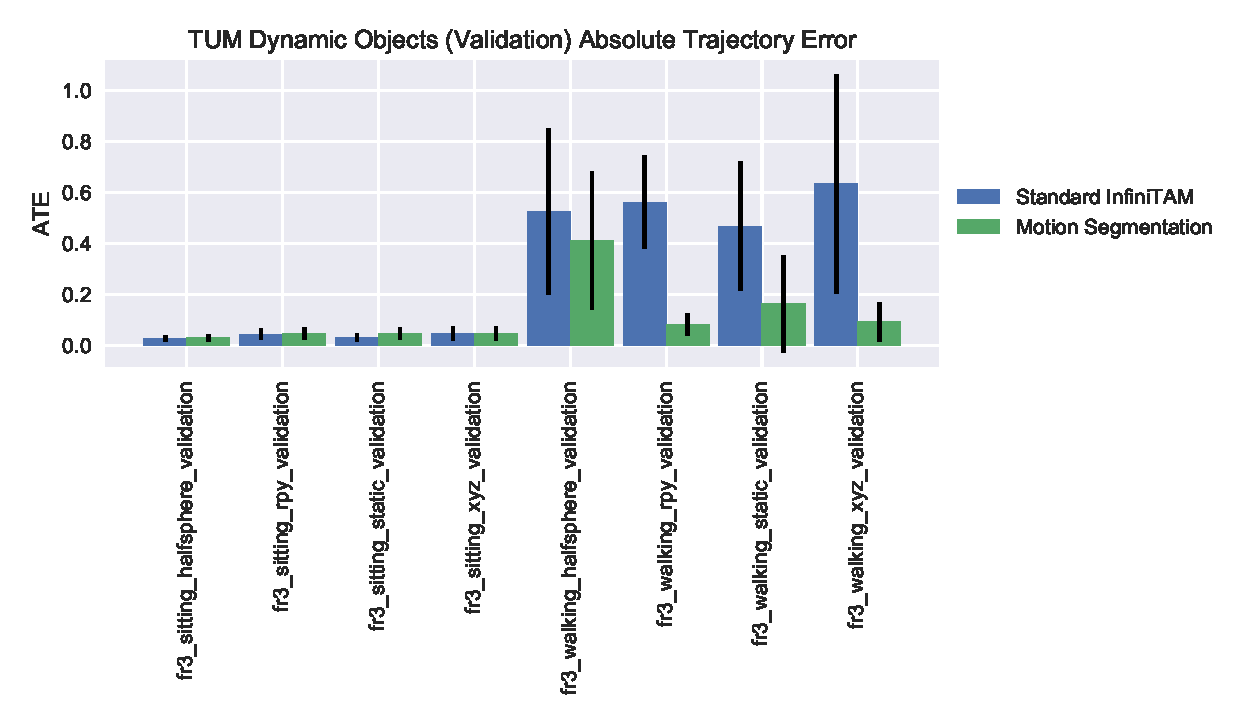
\includegraphics[width=0.95\linewidth]{figures/moseg/ate_validation.eps}
  \caption[Motion Segmentation ATE Validation Set]
  {Absolute Trajectory Error for the TUM Dynamic Scenes
    \textit{Validation} dataset.}
~\label{figure:moseg_ate_validation}
\end{figure}

\subsection{Motion Segmentation figure: RTE results}
In this section, figure: results for the Motion Segmentation system
to complement those outlined in Section~\ref{sec:moseg_quantitative} are given.
The results in this section assess Relative Trajectory Error on the TUM Dynamic
Objects \textit{Validation} set. Quantitative results are given in Table
~\ref{table:moseg_rte_validation} and visualised in Figure
~\ref{figure:moseg_rte_validation}.

\begin{table}[!htbp]
\begin{center}
  \begin{tabular}{l c c}
    \emph{TUM Standard Sequence Name} & \emph{MoSeg} RTE (m) & \emph{Baseline} RTE (m) \\
    \midrule
    \textsf{fr3-sitting-static} & \textbf{0.011} & \textbf{0.011}\\
    \textsf{fr3-sitting-xyz} & \textbf{0.031} & 0.034\\
    \textsf{fr3-sitting-halfsphere} & 0.024 & \textbf{0.022}\\
    \textsf{fr3-sitting-rpy} & 0.051 & \textbf{0.048}\\
    \textsf{fr3-walking-static} & \textbf{0.083} & 0.163\\
    \textsf{fr3-walking-xyz} & \textbf{0.067} & 0.285\\
    \textsf{fr3-walking-halfsphere} & \textbf{0.167} & 0.211\\
    \textsf{fr3-walking-rpy} & \textbf{0.121} & 0.194\\
  \end{tabular}
\end{center}
\caption[Motion Segmentation RTE Validation Set]
{The Relative Trajectory Error (RTE) results (in metres, lower is better) 
achieved by the proposed approach in comparison to the baseline InfiniTAM
~\cite{Prisacariu2014} framework on a variety of the standard sequences from
the TUM RGBD \textit{Validation} dataset~\cite{Sturm2012}. Results are in the
format mean \( \pm \) standard deviation. The better result (by mean) on each
sequence is highlighted in bold.}
~\label{table:moseg_rte_validation}
\end{table}

\begin{figure}[!htbp]
  \centering
  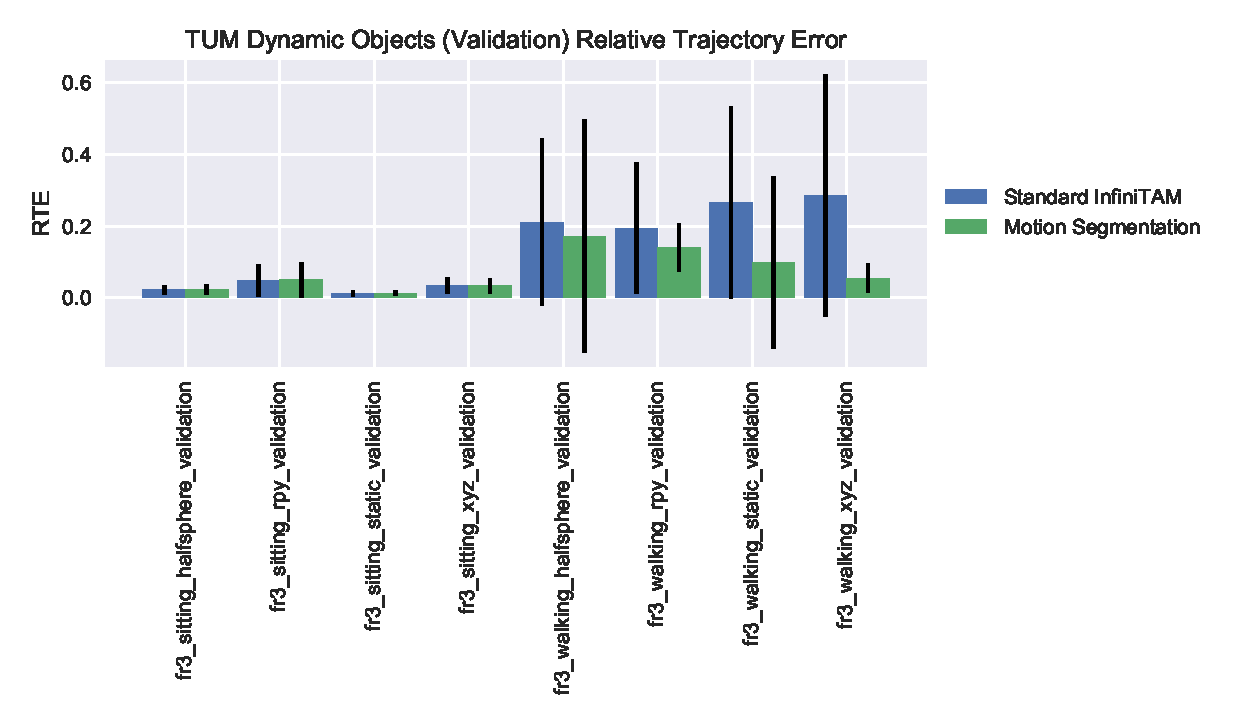
\includegraphics[width=0.95\linewidth]{figures/moseg/rte_validation.eps}
  \caption[Motion Segmentation RTE Validation Set]
  {Relative Trajectory Error for the TUM Dynamic Scenes
    \textit{Validation} dataset.}
~\label{figure:moseg_rte_validation}
\end{figure}